\mychapter{4}{Specific Implementation}
\section{Dimensionality reduction}
Let \textbf{X} = $\displaystyle \{\vect{x}_{1}, \ldots , \vect{x}_{n} \}$
be a data set of n points in a D-dimensional space $\R^{D}$, where D is very large.
Assume that the data points lie on or near an underlying d-dimensional manifold embedded in the high dimensional space $\R^{D}$ where d is much smaller than D.
Dimensionality reduction refers to the process of transforming the high dimensional data 
$\textbf{X}$ into a new data set \textbf{Y} = $\displaystyle \{ \vect{y}_{1}, \ldots, \vect{y}_{n} \}$  of n points in $\R^{d}$ such that each $\vect{y}_{i}$ is a low dimensional representation of  $\vect{x}_{i}$ in the low dimensional space. In addition the transformation must preserve, as much as possible,  the the observed properties in the data such as its underlying geometry. In this case d  is called the intrinsic  dimensionality of the data. 

\subsection{Singular Value Decomposition}
Given any $n \times D$ matrix A with real entries, AA$^{T}$ and A$^{T}$A are 
both real symmetric matrices hence diagonalizable. Hence we can write AA$^{T}$ = VDV$^{T}$ and A$^{T}$A = UDU$^{T}$ where the U and V are orthogonal matrices. The columns of U and V contain the eigen vectors of A$^{T}$A  and AA$^{T}$ respectively. D is a diagonal matrix containing the eigenvalues of AA$^{T}$ which are the same as those for A$^{T}$A. The singular value decomposition (SVD) of A is given by A = U$\Sigma$V$^{T}$ where  $\Sigma$ is a diagonal matrix containing the square roots of the eigen values  of AA$^{T}$ (i.e the singular values of A).


\subsection{Linear dimensionality reduction}
Linear dimensionality reduction techniques find a low dimensional model of the $n \times D$
data matrix $\textbf{X}$ using a linear transformation such as an $n \times d$ orthogonal matrix M where d$<<$D. A common example of a linear technique is principle component analysis (PCA) \cite{JolliffeIT1986PCAa}.
The main assumption in PCA is that the high dimensional data lies on a low dimensional
subspace embedded in the high dimensional space. The best low dimensional subspace that describes the data is then found by minimizing the sum of squared residuals between the orthogonal projection of the data  points onto the estimated low dimensional subspace and the input points (see \eqref{PCA}).



\begin{equation}\label{PCA}
\begin{aligned}
& \underset{M}{\text{minimize}}
& & \sum_{i=1}^{n} \big \lVert \vect{x}_{i} - MM^{T}\vect{x}_{i} \big \rVert_{2}^{2} \\
& \text{subject to}
& & M \in \R^{n \times d} \\
&&& M^{T}M = I.
\end{aligned}
\end{equation}

The solution  to PCA is found via SVD \cite{BishopChristopherM2006Pram, AmericanMathematicalSociety.1939Apat}. The Solution to PCA via SVD is as follows:

\subsection{SVD algorithm}
1. Compute the mean c of the data set \textbf{X} and center
the data so that \textbf{X} = \textbf{X} - c\\
2. Summarize the zero-mean data by computing the covariance matrix $\frac{1}{n}$XX$^{T}$\\
3. Find the spectral decomposition  \textbf{XX}$^{T}$ = VDV$^{T}$ or 
use SVD on centered data, X = U$\Sigma V^{T}$\\
4. Let V$_{d}$ denote the top d columns of V corresponding to the  top r singular values of \textbf{X}\\
5. The optimal point of the optimization problem \eqref{PCA} is M = V$_{d}^{T}$.\\
The low dimensional model \textbf{Y} is obtained by setting \textbf{Y} = V$^{T}$\textbf{X}.\\
In otherwords, the rows of $V^{T}$ (or the columns of V) are an orthonormal basis for transforming \textbf{X} into \textbf{Y}.




\section{Non-linear dimensionality reduction}
The main observation in non-linear dimensionality reduction is that there is no explicit mapping P such that low dimensional model can be obtained via the relationship 
$\textbf{Y} = P\textbf{X}$.

----I need to fill the main steps in a non-linear dimensionality reduction algorithm--------



\section{Nature of our Raw real-world data}
The raw data provided by the Redish Lab is a set of multiple single-unit single-trial
spike trains 
T = $\displaystyle \Set{ \{ t_{i}^{j} \} , 1 \leq i \leq n_{i}, 1 \leq j \leq 32 } $ 
recorded from 32 neurons called  place cells  in the CA1 region of the rat hippocampus.
$\displaystyle  \{t_{i}^{j}\} =  \{t_{1}^{j}, ....., t_{n_{i}}^{j} \} $ represents 
a sequences of n$_{i}$ recorded times at which the spikes of the j$^{th}$ neuron occurred.
The spike trains are of different lengths where t$_{i}^{j}$ represents the i$^{th}$
spike time of the j$^{th}$ neuron.

\section{Preprocessing raw spike train data}
We preprocessed the raw spikes using two methods.
In the first method, the raw spikes were smoothed with a Gaussian kernel to obtain a firing rate. In the second method, we computed the time since the last spike which we call the \textit{previous time}, and then smoothed the previous time with the Laplace Kernel.\\


\subsection{Conversation to a firing rate}
For each neuron labeled j,  we converted the corresponding spike train 
T$^{j}(t) = \displaystyle \sum_{i=1}^{n_{i}} \delta(t-t_{i}^{j}) $ into a firing rate,
 R$^{j}$(t) by replacing K in \eqref{firerate} with the  Gaussian Kernel\\
 K(t) =  $\displaystyle \frac{1}{\sigma \sqrt{2\pi}} e^{-\frac{t^2}{2\sigma^2}} $.
Thus, the firing rate for the j$^{th}$ neuron is given by

\begin{equation} \label{jfirerate}
R^{j}(t) = \sum_{i=1}^{n_{i}}  \frac{1}{\sigma \sqrt{2\pi}} 
e^{-\dfrac{(t_{i_{k}}^{j}  - t_{i_{l}}^{j})^2}{2\sigma^2}} 
\end{equation}

\subsection{Computing the previous time}
Let $\vect{s} = (s_1, s_2, ..., s_n)$  be a vector of n time points representing the different states of the animal's brain  where  $s_1 < s_2 < ... < s_n$. We  define the \textit{previous time} of the j$^{th}$ neuron at the $s_{k}$-th brain state  denoted by , p$^{j}(s_{k})$, as follows:\\
Let t$_{\max}$ = $\max  \Set{ t^{j}_{i} | t^{j}_{i} < s_{k},
1 \leq k \leq n \quad \text{for all} \quad  t^{j}_{i} }.$ Then p$^{j}(s_{k})$ = t$_{\max} - s_{k}.$\\
See example  \eqref{ex1} below.


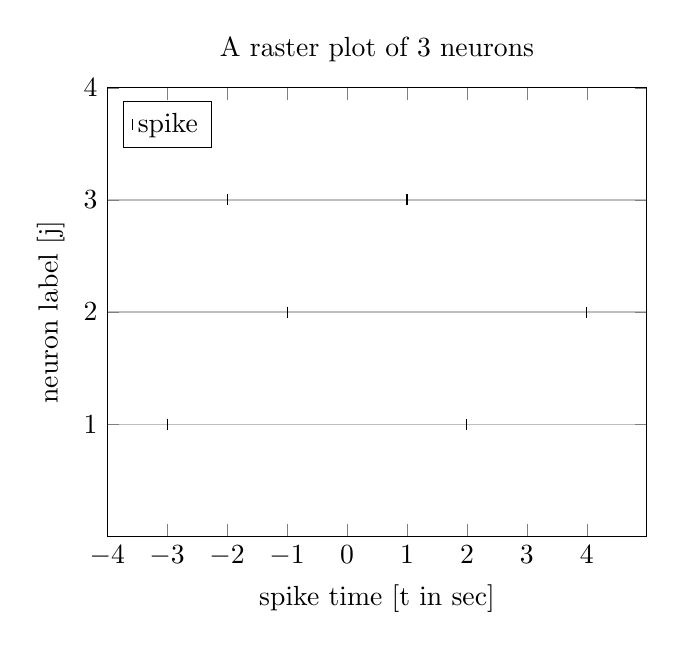
\begin{tikzpicture}
\begin{axis}[
    title={A raster plot of 3 neurons},
    xlabel={spike time [t in sec]},
    ylabel={neuron label [j]},
    xmin=-4, xmax=5,
    ymin=0, ymax= 4,
    xtick={-4, -3,-2,-1,0,1,2,3,4},
    ytick={1,2,3,4},
    legend pos=north west,
    ymajorgrids=true,
    grid style= solid,
]
 
\addplot[
    color=black,
    only marks,
    mark = |
    ]
    coordinates {
    (-3, 1)(-1,2)(-2, 3)(1, 3)(2,1)(4,2)
    };
    \legend{spike}
 
\end{axis}
\end{tikzpicture}


\begin{Ex}\label{ex1}
 \begin{align*}
    p^{j}(s_k=0) &= \begin{bmatrix}
           -3\quad \text{if} \quad j=1 \\
           -1\quad \text{if} \quad j=2\\
           -2\quad  \text{if} \quad  j=3
         \end{bmatrix},
  \end{align*} 
  
  \quad
  
  \begin{align*}
    p^{j}(s_k=2) &= \begin{bmatrix}
           -5\quad \text{if} \quad j=1 \\
           -3\quad \text{if} \quad j=2\\
           -1\quad  \text{if} \quad  j=3
         \end{bmatrix}
  \end{align*} 
  
\end{Ex}





%\begin{tikzpicture}
%%anything after grid adjusts the overall width
%\draw[step=1cm,gray,very thin] (-3.9,-3.9) grid (3.9,3.9);
%\draw[thick] (0,0) -- (0, 3.0) node[anchor=north west] {s$_{k}$ = 0};
%\draw[thick,->] (-3,0) -- (4,0) node[anchor=north west] {spike time};
%\foreach \x in {-3,-2,-1,0,1,2,3}
%    \draw (\x cm,1pt) -- (\x cm,-1pt) node[anchor=north] {$\x$};
%
%\end{tikzpicture}

